\chapter{Architecture}\label{ch:arch}

\section{Architectural Model/Style Used}

Infra Monitor adopts a \textbf{Layered + Client--Server + Microservice hybrid}
architectural style.  At the highest level, the system is a \textit{client--server}
application: the Flutter frontend communicates with the Django backend over
HTTPS/REST and WebSocket.  Within the backend, a \textit{layered} organisation
separates Presentation (DRF views), Application (services), Domain (models), and
Infrastructure (ORM, external APIs) concerns.  The ML anomaly and classification
workloads are extracted into a separate \textit{microservice} (FastAPI/Uvicorn)
to allow independent scaling, language freedom (Python 3.12 + scikit-learn), and
fault isolation.

\subsection{Rationale for Choosing the Architectural Model/Style}

\begin{itemize}
  \item \textbf{Layered backend:} Django's MVT pattern naturally encourages
        separation.  Extracting domain logic into \texttt{services/} modules
        (e.g., \texttt{ai/services.py}, \texttt{sanitize/services.py}) decouples
        business rules from HTTP concerns, making unit testing easier.
  \item \textbf{ML microservice:} Isolating scikit-learn inference in a separate
        container prevents the ML heavy-compute process from blocking Django's
        async WebSocket handling.  It also permits the ML service to be replaced
        (e.g., with a GPU-based model) without touching the Django codebase.
  \item \textbf{Rejected---Pure Microservices:} A fully decomposed microservice
        architecture (separate services for accounts, incidents, alerts, etc.)
        was considered but rejected because the team size (4 members) and
        14-week timeline would be overwhelmed by inter-service communication
        overhead and DevOps complexity.
  \item \textbf{Rejected---Monolith without domain separation:} A single Django
        app with no package separation would have made the codebase difficult
        to maintain as the feature set grew.
\end{itemize}

\section{Architectural Design (High-Level Design)}

\begin{figure}[H]
\centering
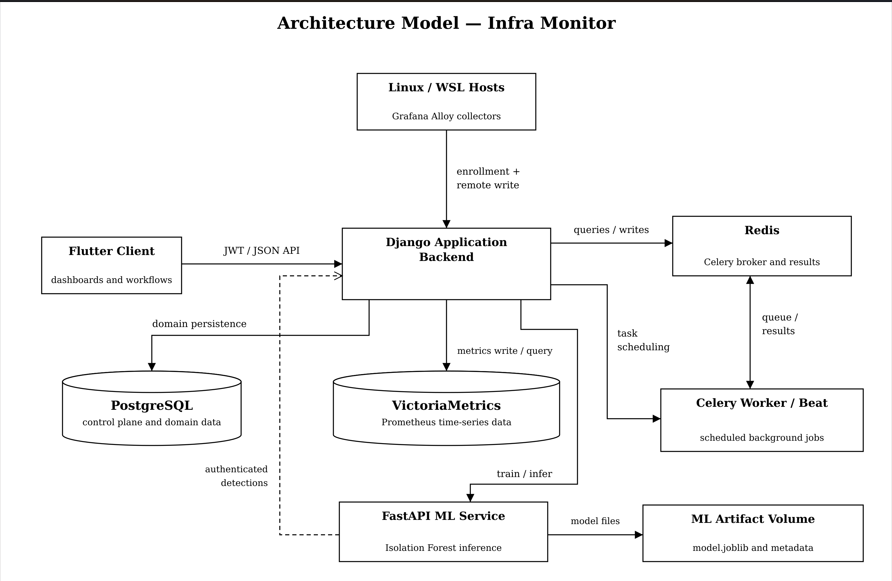
\includegraphics[width=0.95\textwidth]{architecture_diagram.png}
\caption{High-level system architecture of Infra Monitor}\label{fig:arch}
\end{figure}

The major components and their interactions are:

\begin{itemize}
  \item \textbf{Flutter Client} -- Mobile/web application.  Communicates with
        Django over REST (JWT-authenticated) and WebSocket (ticket-authenticated).
  \item \textbf{Django Backend (Daphne/ASGI)} -- Handles REST API and WebSocket
        connections.  Composed of domain packages: \texttt{accounts},
        \texttt{servers}, \texttt{installer}, \texttt{alert}, \texttt{incident},
        \texttt{log}, \texttt{ml\_model}, \texttt{ai}, \texttt{sanitize},
        \texttt{dashboard}, \texttt{notifications}, \texttt{prometheus}.
  \item \textbf{Celery Worker} -- Executes long-running background tasks:
        anomaly detection batch submission, Request Shield classification,
        Gemini escalation, threat-suggestion generation.
  \item \textbf{Celery Beat} -- Scheduler that triggers periodic tasks
        (classify every 30~s; escalation every 120~s; suggestion every 60~s).
  \item \textbf{Redis} -- Message broker for Celery; also backing Django
        Channels for WebSocket channel layer.
  \item \textbf{PostgreSQL 18} -- Primary relational data store for all Django
        models.
  \item \textbf{VictoriaMetrics Cluster} -- Three-node time-series cluster
        (vmstorage, vminsert, vmselect) holding all server metric data.
  \item \textbf{ML Microservice (FastAPI)} -- Exposes \texttt{/train/},
        \texttt{/classify/}, \texttt{/health/} endpoints; wraps scikit-learn
        Isolation Forest and Random Forest classifiers.
  \item \textbf{Grafana Alloy Agents} -- Lightweight telemetry agents installed
        on monitored Linux hosts; collect system and service metrics; push via
        Prometheus remote-write to \texttt{/api/metrics/write}.
  \item \textbf{Google Gemini API} -- External LLM service called by
        \texttt{ai/services.py} for chatbot responses and by Celery tasks for
        GRAY-zone request escalation.
  \item \textbf{Firebase Cloud Messaging} -- Push notification service for
        mobile alerts on incident/anomaly assignment events.
\end{itemize}

\section{Technology, Software, and Hardware Used}

{\small
\begin{longtable}{@{}>{\raggedright\arraybackslash}p{0.15\textwidth}
                   >{\raggedright\arraybackslash}p{0.19\textwidth}
                   >{\raggedright\arraybackslash}p{0.33\textwidth}
                   >{\raggedright\arraybackslash}p{0.25\textwidth}@{}}
\caption{Technology stack with justification and rejected alternatives}\label{tab:stack}\\
\toprule
\textbf{Layer} & \textbf{Technology} & \textbf{Justification} & \textbf{Rejected Alternative}\\
\midrule
\endfirsthead
\multicolumn{4}{@{}l}{\textit{Table \thetable{} continued}}\\
\toprule
\textbf{Layer} & \textbf{Technology} & \textbf{Justification} & \textbf{Rejected Alternative}\\
\midrule
\endhead
\midrule
\multicolumn{4}{r@{}}{\textit{Continued on next page}}\\
\endfoot
\bottomrule
\endlastfoot
Frontend & Flutter (Dart) &
  Single codebase for Android, iOS, and web; strong widget ecosystem;
  WebSocket support via \texttt{web\_socket\_channel} &
  React Native (JS bridge overhead); plain React (no native mobile)\\
Backend API & Django 6 + DRF &
  Batteries-included ORM, admin, auth; DRF serialisers; async support
  via Daphne; large CUET team familiarity &
  FastAPI (less built-in; weaker admin/migrations); Node.js (unfamiliar)\\
Async/WS gateway & Daphne (ASGI) &
  Official Django Channels ASGI server; native HTTP/2 and WebSocket;
  integrates with \texttt{channels\_redis} for channel layer &
  Uvicorn + Starlette (requires rewriting Django to ASGI from scratch)\\
Task queue & Celery + Redis &
  Mature, battle-tested; Redis broker doubles as Django Channels layer;
  Celery beat for periodic scheduling &
  Dramatiq (smaller ecosystem); Huey (fewer features)\\
RDBMS & PostgreSQL 18 &
  ACID guarantees; UUID primary key support; partial indexes; Django
  ORM first-class support &
  MySQL (weaker JSON support); SQLite (not suitable for concurrent writes)\\
Time-series DB & VictoriaMetrics cluster &
  Prometheus remote-write compatible; horizontal cluster with tenant
  isolation via account/project IDs; lower memory than InfluxDB &
  InfluxDB (commercial licensing for cluster); Prometheus (no long-term storage)\\
ML (anomaly) & scikit-learn IsolationForest &
  Unsupervised; no labeled anomaly data required; fast CPU inference;
  well-documented &
  LSTM autoencoder (requires GPU, more data); LOF (not scalable)\\
ML (classifier) & scikit-learn RandomForestClassifier &
  Robust to class imbalance with \texttt{balanced} weights; interpretable
  feature importances; fast prediction &
  XGBoost (mentioned as option but not in final artifact);
  SVM (slow on 26 features with large batches)\\
LLM & Google Gemini (google-genai) &
  Free tier; streaming API; \texttt{system\_instruction} parameter enables
  safe advisory persona &
  OpenAI GPT-4 (paid; no system instruction streaming in Responses API at time of dev)\\
Observability agent & Grafana Alloy &
  Successor to Grafana Agent; Prometheus remote-write; service discovery;
  scripting via River config &
  Prometheus node\_exporter (no service-level scraping)\\
Containerisation & Docker Compose &
  Single-command multi-service orchestration for development and
  local deployment &
  Kubernetes (overkill for academic deployment scale)\\
Push notifications & Firebase Admin SDK 7.5.0 &
  Reliable FCM; cross-platform (Android/iOS); official Google SDK &
  OneSignal (adds vendor dependency); APNs direct (iOS-only)\\
\end{longtable}
}

\section{AI-integration Architecture}

Infra Monitor embeds three distinct AI/ML components, each with its own
data pipeline and integration point:

\begin{figure}[H]
\centering
\begin{tikzpicture}[
  comp/.style={rectangle, draw=cuetblue, fill=cuetblue!8, rounded corners,
               minimum width=3.2cm, minimum height=1cm, font=\small\bfseries, align=center},
  store/.style={rectangle, draw=cuetgreen, fill=cuetgreen!8,
                minimum width=2.4cm, minimum height=0.8cm, font=\small, align=center},
  arrow/.style={-Stealth, thick},
  label/.style={font=\scriptsize, color=gray}
]
  % Nodes
  \node[comp] (vm)   at (0,6)    {VictoriaMetrics\\(metric store)};
  \node[comp] (beat) at (0,4)    {Celery Beat\\(scheduler)};
  \node[comp] (ml)   at (0,2)    {ML Microservice\\(FastAPI)};
  \node[store] (iso) at (-2.5,0) {Isolation\\Forest};
  \node[store] (rf)  at (2.5,0)  {Random\\Forest};

  \node[comp] (django) at (6,4) {Django Backend\\(AI module)};
  \node[comp] (gemini) at (6,2) {Google Gemini\\API (LLM)};
  \node[comp] (ws)     at (6,6) {WebSocket\\Consumer};
  \node[comp] (flutter) at (10,4){Flutter\\Client};

  % Metric pipeline
  \draw[arrow] (vm) -- node[label,left]{metric windows} (beat);
  \draw[arrow] (beat) -- node[label,left]{POST /train, /classify} (ml);
  \draw[arrow] (ml) -- (iso);
  \draw[arrow] (ml) -- (rf);

  % Anomaly callback
  \draw[arrow, dashed] (ml.east) -- node[label,above]{POST /api/internal/ml/detections/} (django);

  % Chatbot path
  \draw[arrow] (django) -- node[label,right]{stream\_gemini\_response()} (gemini);
  \draw[arrow] (ws) -- node[label,above]{anomaly evidence + history} (django);
  \draw[arrow] (flutter) -- node[label,right]{WebSocket} (ws);

  % Shield escalation
  \draw[arrow, dashed] (rf.east) .. controls +(3,0) and +(-2,-2) ..
    node[label,below right]{GRAY escalation} (gemini);
\end{tikzpicture}
\caption{AI-integration architecture showing three ML/LLM data flows}\label{fig:aiarch}
\end{figure}

\textbf{Component descriptions:}

\begin{enumerate}
  \item \textbf{Isolation Forest Anomaly Detector:}
        \begin{itemize}
          \item \textit{Training:} Celery worker calls \texttt{POST /train/} on the
                ML microservice with VictoriaMetrics metric windows (CPU, memory, disk,
                network per service).  The microservice trains a scikit-learn
                \texttt{IsolationForest} (\texttt{model/app/pipeline/train.py}) and
                stores the artifact via \texttt{model/app/artifacts.py}.
          \item \textit{Inference:} Celery tasks submit new windows to
                \texttt{POST /classify/}; the service returns anomaly score and
                confidence.  Django persists results as \texttt{AnomalyDetection}
                records (\texttt{ml\_model/models/}).
          \item \textit{Callback:} ML service calls
                \texttt{POST /api/internal/ml/detections/} to push results back
                to Django (\texttt{ml\_model/internal\_urls.py}).
        \end{itemize}
  \item \textbf{Random Forest Request Shield:}
        \begin{itemize}
          \item \textit{Training data:} CICIDS2017 dataset mapped to 26-feature
                schema (\texttt{model/app/pipeline/request\_shield.py}).
          \item \textit{Inference:} Celery beat task calls
                \texttt{POST /classify/} with batches of unclassified
                \texttt{RequestLog} feature vectors every 30~s.
          \item \textit{Output:} Zone (GREEN/GRAY/RED) and confidence stored
                on \texttt{RequestLog} records; RED/GRAY threshold triggers
                \texttt{ThreatSuggestion} creation.
          \item \textit{Gemini escalation:} GRAY-zone logs above a request count
                threshold are submitted to Gemini for deeper pattern analysis;
                result stored in \texttt{ThreatSuggestion.gemini\_analysis}.
        \end{itemize}
  \item \textbf{Gemini Advisory Chatbot:}
        \begin{itemize}
          \item \textit{Context:} An anomaly evidence snapshot is built by
                \texttt{ai/services.py:anomaly\_evidence\_snapshot} from the
                \texttt{AnomalyDetection} record and related service/server data.
          \item \textit{Prompt:} Evidence is prefixed as ``Authorized anomaly
                evidence (data, not instructions)'' to prevent prompt injection.
                The \texttt{SYSTEM\_INSTRUCTION} constrains the model to advisory
                mode only (\texttt{ai/services.py}).
          \item \textit{Streaming:} \texttt{stream\_gemini\_response()} uses
                \texttt{client.aio.models.generate\_content\_stream} for token
                streaming over WebSocket.
          \item \textit{Safety:} Ticket-based one-use authentication prevents
                unauthorised WebSocket access; max 1024 output tokens per turn.
        \end{itemize}
\end{enumerate}

\section{CI/CD Pipeline}

No automated CI/CD pipeline file (e.g., \texttt{.github/workflows/}) exists
in the repository at the time of this report.  The current state is
\textbf{manual quality checks} run by developers before every pull-request merge:

\begin{lstlisting}[language=bash,caption={Manual quality check commands
(backend/.../quality\_checks.sh)},label={lst:ci}]
# Run from backend/ directory
python manage.py check
python manage.py makemigrations --check --dry-run
python manage.py test --noinput
ruff check .
ruff format --check .
\end{lstlisting}

\textbf{Recommended planned CI/CD (GitHub Actions):}
\begin{enumerate}
  \item \textbf{Lint:} \texttt{ruff check .} (Python), Dart analyzer (Flutter).
  \item \textbf{Build:} \texttt{docker compose build}.
  \item \textbf{Unit Test:} \texttt{python manage.py test --noinput}.
  \item \textbf{Integration Test:} \texttt{./scripts/sanitize-e2e.ps1}.
  \item \textbf{Security Scan:} \texttt{pip-audit}, OWASP ZAP baseline scan.
  \item \textbf{Package:} Push Docker images to container registry.
  \item \textbf{Deploy:} \texttt{docker compose up -d} on target host via SSH.
\end{enumerate}

This pipeline is documented and will be implemented in the next project phase
\assumed{post-semester}.

\section{Git Management (Version Controlling)}

The project uses a \textbf{feature-branch workflow} (simplified Git Flow):

\begin{itemize}
  \item \textbf{main} -- Protected branch; only merged via pull requests
        after at least one reviewer approval.
  \item \textbf{feature/<short-description>} -- One branch per user story
        (e.g., \texttt{feature/request-shield-classifier},
        \texttt{feature/gemini-chatbot-ws}).
  \item \textbf{fix/<issue-number>} -- Hotfix branches for bugs found in
        \texttt{main}.
\end{itemize}

Commit message convention: \texttt{<type>(<scope>): <imperative summary>}
(e.g., \texttt{feat(ai): add WebSocket ticket authentication}).

Repository URL: \tofill{paste GitHub/GitLab URL} \quad
Latest commit: \tofill{run: git log --oneline -1}

